% !TeX program = xelatex
\documentclass[a4paper,10pt]{article}

% ============================================================================
% កញ្ចប់បណ្ណាល័យ (Packages) – តាមលំនាំស្តង់ដារ អនុវិទ្យាល័យព្រះក្រសាំង (ls_plan.tex)
% បរិបទ៖ ថ្នាក់រៀនគ្មានស្លាយ LCD – បង្រៀនដោយប្រើក្ដារខៀន សៀវភៅគោល និងសន្លឹកកិច្ចការស-ខ្មៅ
% ============================================================================
\usepackage[a4paper, left=0.95cm, right=0.95cm, top=0.85cm, bottom=0.92cm, footskip=0.52cm]{geometry}
\usepackage{amsmath}
\usepackage{unicode-math}
\usepackage{fontspec}
\usepackage{array, longtable, multirow, colortbl}
\usepackage[table]{xcolor}
\usepackage{enumitem}
\usepackage{pifont}
\usepackage{fancyhdr}
\usepackage{tikz}
\usetikzlibrary{calc, arrows.meta, positioning, babel}

\makeatletter
\let\@expl@@@mark@update@singlecol@structures@@\relax
\makeatother

\providecommand{\NGSFindFonts}{%
  \IfFileExists{C:/Windows/Fonts/cambria.ttc}{%
    \def\NGSSysPath{C:/Windows/Fonts/}%
    \def\NGSUserPath{C:/Users/KIT/AppData/Local/Microsoft/Windows/Fonts/}%
  }{%
    \IfFileExists{./fonts/KhmerOSsiemreap.ttf}{\def\NGSSysPath{./fonts/}\def\NGSUserPath{./fonts/}}{%
    \IfFileExists{../fonts/KhmerOSsiemreap.ttf}{\def\NGSSysPath{../fonts/}\def\NGSUserPath{../fonts/}}{%
    \IfFileExists{../../fonts/KhmerOSsiemreap.ttf}{\def\NGSSysPath{../../fonts/}\def\NGSUserPath{../../fonts/}}{%
    \IfFileExists{../../../fonts/KhmerOSsiemreap.ttf}{\def\NGSSysPath{../../../fonts/}\def\NGSUserPath{../../../fonts/}}{%
    \IfFileExists{../../../../fonts/KhmerOSsiemreap.ttf}{\def\NGSSysPath{../../../../fonts/}\def\NGSUserPath{../../../../fonts/}}{%
    \IfFileExists{../../../../../fonts/KhmerOSsiemreap.ttf}{\def\NGSSysPath{../../../../../fonts/}\def\NGSUserPath{../../../../../fonts/}}{%
    \IfFileExists{../../../../../../fonts/KhmerOSsiemreap.ttf}{\def\NGSSysPath{../../../../../../fonts/}\def\NGSUserPath{../../../../../../fonts/}}{%
      \def\NGSSysPath{../../../../../../../fonts/}\def\NGSUserPath{../../../../../../../fonts/}%
    }}}}}}}%
  }%
}
\NGSFindFonts

\setmathfont[Path={\NGSSysPath}, FontIndex=1, Scale=1.02]{cambria.ttc}
\defaultfontfeatures{Ligatures=TeX}

\setmainfont[
  Path={\NGSUserPath},
  Extension=.ttf,
  Script=Khmer,
  BoldFont={KhmerOSsiemreap},
  BoldFeatures={FakeBold=1.8},
  ItalicFont={KhmerOSsiemreap},
  ItalicFeatures={FakeSlant=0.25},
  BoldItalicFont={KhmerOSsiemreap},
  BoldItalicFeatures={FakeBold=1.8, FakeSlant=0.25}
]{KhmerOSsiemreap}

\newfontfamily\muol[Path={\NGSUserPath}, Extension=.ttf, Script=Khmer]{KhmerOSmuollight}
\newfontfamily\TimesEn[Path={\NGSSysPath}, Extension=.ttf, BoldFont={timesbd}, ItalicFont={timesi}, BoldItalicFont={timesbi}]{times}
\newfontfamily\NagaBold[Path={\NGSUserPath}, Extension=.ttf]{AKbalthom Naga Bold}
\newfontfamily\CalibriFont[Path={\NGSSysPath}, Extension=.ttf]{calibri}
\newfontfamily\Tacteing[Path={\NGSUserPath}]{TACTENG.TTF}
\newfontfamily\CourierBullet[Path={\NGSSysPath}, Extension=.ttf]{cour}
\newcommand{\wcirc}{{\CourierBullet\fontsize{9.5pt}{11pt}\selectfont o}}

\XeTeXlinebreaklocale "km"
\XeTeXlinebreakskip = 0pt plus 1pt minus 0.1pt

\definecolor{stepgray}{HTML}{D9D9D9}
\definecolor{headgray}{HTML}{F2F2F2}
\definecolor{boxgray}{HTML}{D9D9D9}
\definecolor{darkred}{HTML}{C00000}
\definecolor{red5e}{HTML}{FF0000}

\pagestyle{fancy}
\fancyhf{}
\renewcommand{\headrulewidth}{0pt}
\fancyfoot[R]{\CalibriFont\fontsize{11pt}{13pt}\selectfont\thepage}

\setlength{\parindent}{0pt}
\setlength{\parskip}{0pt}
\setlength{\tabcolsep}{3.8pt}

\newcolumntype{L}[1]{>{\raggedright\arraybackslash}p{#1}}

\newcommand{\en}[1]{{\TimesEn #1}}
\newcommand{\enbf}[1]{{\TimesEn\textbf{#1}}}
\newcommand{\unit}[1]{\,\text{\en{#1}}}
\newcommand{\fiveE}[1]{{\NagaBold\fontsize{9.5pt}{13pt}\selectfont\textcolor{red5e}{#1}}}
\newcommand{\timenote}[1]{\textcolor{darkred}{\textit{#1}}}
\newcommand{\graybox}[1]{\colorbox{boxgray}{\strut\hspace{2pt}#1\hspace{2pt}}}
\newcommand{\ditem}{\tikz[baseline=-0.5ex]\fill (0,0.42ex) -- (0.42ex,0) -- (0,-0.42ex) -- (-0.42ex,0) -- cycle;\hspace{0.3em}}
\newcommand{\cnum}[1]{{\fontsize{10.5pt}{12pt}\selectfont\ding{\numexpr171+#1\relax}}\hspace{0.2em}}
\newcommand{\cfig}[1]{\par\vspace{4pt}{\centering #1\par}\vspace{4pt}}
\newcommand{\stepheader}[1]{\multicolumn{3}{|c|}{\cellcolor{stepgray}\muol #1} \\* \noalign{\hrule height 0.4pt}}
\newcommand{\khmflourish}{{\Tacteing\fontsize{36pt}{14pt}\selectfont\raisebox{-5pt}{3}}}

% ============================================================================
% ម៉ាក្រូរូបភាពគរុកោសល្យស-ខ្មៅ (Proportional B&W TikZ Diagrams)
% ============================================================================

% ១. E1 Engage: បរិមាត្រត្រីកោណ ABC (ទំ.៥៦) + អន្ទាក់ដឺក្រេពហុធា y^3 + 4y^4x + 7 + y
\newcommand{\figEngageALGThree}{%
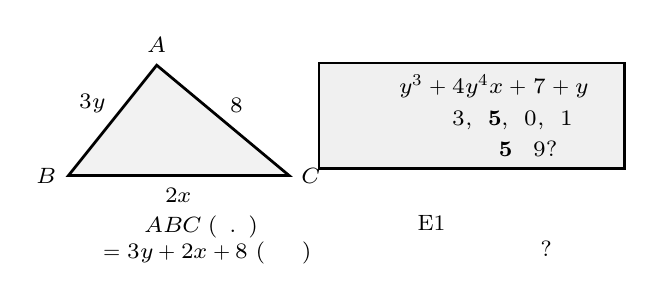
\begin{tikzpicture}[scale=0.80, every node/.style={font=\footnotesize, text=black}]
  % ឆ្វេង៖ ត្រីកោណ ABC (ទំ.៥៦)
  \begin{scope}[shift={(0,0)}]
    \coordinate (B) at (0.10,0.40);
    \coordinate (C) at (3.60,0.40);
    \coordinate (A) at (1.50,2.15);
    \draw[black, line width=1.0pt, fill=gray!10] (A) -- (B) -- (C) -- cycle;
    \node[above=1pt] at (A) {$A$};
    \node[left=1pt] at (B) {$B$};
    \node[right=1pt] at (C) {$C$};
    \node[above left=-1pt] at ($(A)!0.5!(B)$) {$3y$};
    \node[above right=-1pt] at ($(A)!0.5!(C)$) {$8$};
    \node[below=1pt] at ($(B)!0.5!(C)$) {$2x$};
    \node[anchor=north, text width=3.55cm, align=center] at (1.85,-0.08) {ត្រីកោណ $ABC$ (ទំ.៥៦)៖\\បរិមាត្រ $= 3y + 2x + 8$ (ត្រីធា)};
  \end{scope}

  % ស្ដាំ៖ អន្ទាក់ដឺក្រេនៃពហុធា vs ដឺក្រេនៃឯកធា
  \begin{scope}[shift={(4.35,0)}]
    \node[draw=black, line width=0.9pt, fill=gray!12, text width=3.60cm, align=center, inner sep=4pt] at (2.15,1.35) {
      ពហុធា៖ $y^3 + 4y^4x + 7 + y$\\[2pt]
      ដឺក្រេតាមតួ៖ $3,\; \mathbf{5},\; 0,\; 1$\\[2pt]
      តើដឺក្រេពហុធាស្មើ $\mathbf{5}$ ឬ $9$?
    };
    \node[anchor=north, text width=3.80cm, align=center] at (2.15,-0.08) {បេសកកម្ម E1៖ យកដឺក្រេតួខ្ពស់បំផុត\\ឬបូកដឺក្រេគ្រប់តួចូលគ្នា?};
  \end{scope}
\end{tikzpicture}}

% ២. E4 Elaborate: តារាងជួរឈរតម្រឹមដឺក្រេជាមួយចន្លោះ 0x និងការដូរសញ្ញាដក (ទំ.៥៩)
\newcommand{\figColumnALGThree}{%
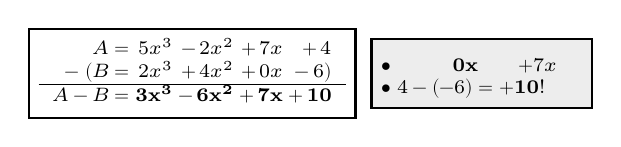
\begin{tikzpicture}[every node/.style={font=\scriptsize, text=black}]
  \node[draw=black, line width=0.9pt, fill=white, inner sep=3.5pt] (col) at (0,0) {%
    $\begin{array}{r@{\;}r@{\;}r@{\;}r@{\;}r}
      A = & 5x^3 & -\,2x^2 & +\,7x & +\,4 \\
      -\;(B = & 2x^3 & +\,4x^2 & +\,0x & -\,6) \\
      \hline
      A - B = & \mathbf{3x^3} & \mathbf{-\,6x^2} & \mathbf{+\,7x} & \mathbf{+\,10}
    \end{array}$%
  };
  \node[draw=black, line width=0.75pt, fill=gray!14, text width=2.55cm, align=left, inner sep=3.5pt, right=5pt of col] {
    \textbf{គន្លឹះការពារកំហុស៖}\\
    $\bullet$ ដាក់ខ្ទង់ $\mathbf{0x}$ ក្រោម $+7x$\\
    $\bullet$ $4 - (-6) = \mathbf{+10}$!
  };
\end{tikzpicture}}

\begin{document}
\fontsize{10pt}{15.2pt}\selectfont

% -------------------- ក្បាលកិច្ចតែងការ (Header) --------------------
\begin{center}
  {\muol\fontsize{11pt}{16pt}\selectfont ព្រះរាជាណាចក្រកម្ពុជា}\\[2pt]
  {\muol\fontsize{10pt}{15pt}\selectfont ជាតិ សាសនា ព្រះមហាក្សត្រ}\\[1pt]
  \khmflourish
\end{center}

\vspace{-28pt}
{\muol\fontsize{9.5pt}{12.5pt}\selectfont
មន្ទីរអប់រំ យុវជន និងកីឡា ខេត្តកំពង់ធំ\\
ការិយាល័យអប់រំ យុវជន និងកីឡា ស្រុកកំពង់ស្វាយ\\
អនុវិទ្យាល័យព្រះក្រសាំង}

\vspace{1pt}
\begin{center}
  {\muol\fontsize{10pt}{14pt}\selectfont កិច្ចតែងការបង្រៀន}
\end{center}
\vspace{0pt}

% -------------------- ព័ត៌មានទូទៅ (Metadata) --------------------
{\renewcommand{\arraystretch}{0.95}
\hspace*{4.05cm}%
\begin{tabular}{@{}l l l@{}}
  - \hspace{0.35cm} មុខវិជ្ជា & : & គណិតវិទ្យា ថ្នាក់ទី៨ \\
  - \hspace{0.35cm} ចំណងជើងមេរៀន & : & មេរៀនទី៥ កន្សោមពីជគណិត \\
  - \hspace{0.35cm} ចំណងជើងរង & : & ២.១--២.៣ សញ្ញាណពហុធា ដឺក្រេ និងវិធីបូក-ដកពហុធា (ទំ.៥៦--៥៩) \\
  - \hspace{0.35cm} រយៈពេល & : & ១ ម៉ោងសិក្សា (៥០ នាទី) \\
  - \hspace{0.35cm} បង្រៀនដោយ & : & ហុក ប៊ុនថែន \\
  - \hspace{0.35cm} កាលបរិច្ឆេទ & : & ថ្ងៃចន្ទ ១៣រោច ខែកត្តិក ព.ស.២៥៧០ (៧ ធ្នូ ២០២៦) \\
\end{tabular}
}

\vspace{1pt}

% -------------------- I. វត្ថុបំណង --------------------
\textbf{I.} {\muol វត្ថុបំណង}\\[1pt]
\hspace*{0.55cm}%
\begin{tabular}{@{}l l L{14.2cm}@{}}
  \wcirc \hspace{0.25cm} វិជ្ជាសម្បទា & : & សិស្សប្រាប់បានត្រឹមត្រូវនូវនិយមន័យ \textbf{ពហុធា} \textbf{ទ្វេធា} \textbf{ត្រីធា} \textbf{ដឺក្រេនៃពហុធា} (ដឺក្រេរបស់តួដែលមានដឺក្រេខ្ពស់ជាងគេ) ការរៀបតាមលំដាប់កើន/ចុះ និងវិធានបូក-ដកពហុធាតាមជួរដេក និងជួរឈរ តាមសៀវភៅគោល ទំ.៥៦--៥៩ ។ \\
  \wcirc \hspace{0.25cm} បំណិនសម្បទា & : & សិស្សកំណត់តួ អថេរ និងដឺក្រេនៃពហុធា រៀបពហុធាតាមលំដាប់កើន/ចុះ និងគណនាផលបូក-ផលដកពហុធាដោយប្រើ \textbf{តារាងជួរឈរតម្រឹមដឺក្រេមានខ្ទង់សូន្យ ($0x$)} និងការបើកវង់ក្រចកមុខសញ្ញាដកបានត្រឹមត្រូវ ។ \\
  \wcirc \hspace{0.25cm} ចរិយាសម្បទា & : & សិស្សមានរបៀបរៀបរយក្នុងការតម្រឹមខ្ទង់ឯកធាដូចគ្នា ប្រុងប្រយ័ត្នចំពោះសញ្ញាដកនៅមុខវង់ក្រចក និងសហការពិភាក្សាដៃគូយ៉ាងសកម្ម ។ \\
\end{tabular}

\vspace{1pt}

% -------------------- II. សម្ភារៈឧបទេស --------------------
\textbf{II.} {\muol សម្ភារៈឧបទេស}\\[1pt]
\hspace*{0.55cm}$\bullet$ \hspace{0.35cm} សៀវភៅសិក្សាគោលគណិតវិទ្យាថ្នាក់ទី៨ (ទំ.៥៦--៥៩ និងទំ.៧២--៧៣) ក្ដារខៀន ដីស បន្ទាត់ និងសន្លឹកកិច្ចការសិស្សស-ខ្មៅ (\en{Worksheet\_ALG53} ចំនួន ២ ទំព័រ \en{A4} ដោយគ្មានស្លាយ \en{LCD}) ។

\vspace{1pt}

% -------------------- III. វិធីសាស្រ្តបង្រៀន --------------------
\textbf{III.} {\muol វិធីសាស្រ្តបង្រៀន}\\[1pt]
\hspace*{0.55cm}$\bullet$ \hspace{0.35cm} គោលវិធីសិស្សមជ្ឈមណ្ឌលតាមគំរូ \en{5Es} រួមបញ្ចូល \textbf{តារាងជួរឈរតម្រឹមដឺក្រេមានខ្ទង់សូន្យ និងរបាំងការពារសញ្ញាដកមុខវង់ក្រចក} (\en{Degree-Aligned Columnar Ledger \& Minus-Bracket Sign-Guard}; \en{Theba et al., 2024; Aydin-G\"u\c{c} \& Ayg\"un, 2021}) ។

\vspace{2pt}

% -------------------- IV. ដំណើរការបង្រៀន --------------------
\textbf{IV.} {\muol ដំណើរការបង្រៀន}\\[-6pt]

{\renewcommand{\arraystretch}{1.15}
\begin{longtable}{|L{5.50cm}|L{7.90cm}|L{4.80cm}|}
\hline
\multicolumn{1}{|c|}{\cellcolor{headgray}\muol សកម្មភាពគ្រូ} &
\multicolumn{1}{c|}{\cellcolor{headgray}\muol ខ្លឹមសារមេរៀន} &
\multicolumn{1}{c|}{\cellcolor{headgray}\muol សកម្មភាពសិស្ស} \\[2pt]
\hline
\endfirsthead

\hline
\multicolumn{1}{|c|}{\cellcolor{headgray}\muol សកម្មភាពគ្រូ} &
\multicolumn{1}{c|}{\cellcolor{headgray}\muol ខ្លឹមសារមេរៀន} &
\multicolumn{1}{c|}{\cellcolor{headgray}\muol សកម្មភាពសិស្ស} \\[2pt]
\hline
\endhead

\hline
\endfoot

% ==================== ជំហានទី១ (2min) ====================
\stepheader{ជំហានទី១ ៖ រដ្ឋបាលថ្នាក់ (២ នាទី)}
$\bullet$ ពិនិត្យអវត្តមាន សណ្ដាប់ធ្នាប់ អនាម័យ និងសៀវភៅគោល \par\vspace{1pt}
$\bullet$ ចែកសន្លឹកកិច្ចការស-ខ្មៅ \en{Worksheet\_ALG53} ដល់សិស្សគ្រប់គ្នា
&
$\bullet$ វត្តមានសិស្ស ឯកសណ្ឋាន និងសណ្ដាប់ធ្នាប់ថ្នាក់រៀន \par
$\bullet$ សន្លឹកកិច្ចការសិស្ស \en{Worksheet\_ALG53} (ទំព័រ ១--២) លើតុរៀងៗខ្លួន
&
$\circ$ ប្រធានថ្នាក់រាយការណ៍អវត្តមាន \par
$\circ$ សរសេរឈ្មោះលើសន្លឹកកិច្ចការ \\
\hline

% ==================== ជំហានទី២ (9min) ====================
\stepheader{ជំហានទី២ ៖ កែកិច្ចការផ្ទះ រំលឹកមេរៀនចាស់ និងភ្ជាប់បញ្ហាថ្មី (៩ នាទី)}
\ditem \textbf{កែកិច្ចការផ្ទះ ($\le 3\unit{min}$)៖} \par
$\bullet$ ហៅសិស្ស ១ រូបឡើងកែលំហាត់ ៣ខ (ទំ.៧២) និងប្រតិបត្តិចែក (ទំ.៥៦) លើក្ដារខៀន
&
\textbf{កំណែកិច្ចការផ្ទះ (ទំ.៧២ និងទំ.៥៦)៖} \par
១) ៣ខ៖ $\frac{3}{2}x^4y^4t + 2x^4y^4t - x^4y^2t = \mathbf{\frac{7}{2}x^4y^4t - x^4y^2t}$ \textit{(តួទី៣ មាន $y^2$ មិនអាចបូកបញ្ចូលជាមួយ $y^4$ បានទេ!)} ។ \par
២) $\dfrac{ax^7b^5}{ax^5b^3} = \mathbf{x^2b^2}$ ។
&
$\circ$ ផ្ទៀងផ្ទាត់ថាហេតុអ្វី $\frac{7}{2}x^4y^4t - x^4y^2t$ មិនអាចបង្រួមតទៀតបាន \\[3pt]

\ditem \textbf{រំលឹកមេរៀនចាស់ ($3\unit{min}$)៖} \par
$\bullet$ សួររំលឹកពីការបូក-ដកឯកធាដូចគ្នា ដឺក្រេនៃឯកធា $4y^4x$ និងការលុបវង់ក្រចកមុខសញ្ញាដក $-(a - b)$
&
\textbf{សំណួររំលឹកមូលដ្ឋានគ្រឹះ៖} \par
១) ឯកធា $4y^4x = 4y^4x^1$ មានដឺក្រេ $4 + 1 = \mathbf{5}$ ។ \par
២) ច្បាប់សញ្ញាមុខវង់ក្រចក៖ $-(x^2 + 4x - 6) = -x^2 - 4x + 6$ ។
&
$\circ$ ឆ្លើយរំលឹកការដូរសញ្ញាគ្រប់តួក្នុងវង់ក្រចកពេលមានសញ្ញាដកនៅពីមុខ \\[3pt]

\fiveE{E1 - Engage} \timenote{(3 នាទី)} \par\vspace{1pt}
$\bullet$ គូសត្រីកោណ $ABC$ (ទំ.៥៦) លើក្ដារខៀន និងបង្ហាញពហុធា $y^3 + 4y^4x + 7 + y$ រួចឱ្យសិស្សគូសធីកការទស្សន៍ទាយក្នុងផ្នែកទី១
&
\textbf{ស្ថានភាពភ្ជាប់បញ្ហា៖ បរិមាត្រត្រីកោណ និងអន្ទាក់ដឺក្រេនៃពហុធា!} \par
បរិមាត្រត្រីកោណ $ABC$ គឺ $3y + 2x + 8$ (ផលបូកឯកធាមិនដូចគ្នា ហៅថា \textbf{ពហុធា}) ។ ចុះចំពោះពហុធា $y^3 + 4y^4x + 7 + y$ (ទំ.៥៧)៖ \par
\hspace*{0.3em}– \textbf{សំណួរបេសកកម្ម៖} «តើដឺក្រេនៃពហុធានេះស្មើ $4$ (លេខនិទស្សន្តធំបំផុតលើរូប) ស្មើ $\mathbf{5}$ (ដឺក្រេតួខ្ពស់បំផុត $4y^4x^1$) ឬស្មើ $9$ (បូកដឺក្រេគ្រប់តួ $3+5+0+1$)?»
&
$\circ$ សង្កេតកន្សោមបរិមាត្រ $3y+2x+8$ \par
$\circ$ គូសធីកការទស្សន៍ទាយមុនរៀន ($4, 5$ ឬ $9$) ក្នុងផ្នែកទី១ នៃសន្លឹកកិច្ចការ \\[3pt]

& \cfig{\figEngageALGThree} & \\
\hline

% ==================== ជំហានទី៣ (17min) ====================
\stepheader{ជំហានទី៣ ៖ មេរៀនថ្មី — សញ្ញាណពហុធា ដឺក្រេ និងវិធីបូក-ដកពហុធា (១៧ នាទី)}
\fiveE{E2 - Explore} \timenote{(11 នាទី)} \par\vspace{1pt}
\ditem \textbf{សកម្មភាពទី១៖ ចំណាត់ថ្នាក់ពហុធា តួ និងដឺក្រេពហុធា ($5.5\unit{min}$)៖} \par
$\bullet$ ឱ្យសិស្សធ្វើការជាដៃគូលើ \textbf{ផ្នែកទី២ (ក)} នៃ \en{Worksheet\_ALG53} ដើម្បីញែកទ្វេធា/ត្រីធា មិនមែនពហុធា និងរកដឺក្រេខ្ពស់បំផុត
&
\textbf{ការរុករកទី១ (២.១ សញ្ញាណ និង ២.២ ដឺក្រេពហុធា ទំ.៥៦--៥៨)៖} \par
$\bullet$ ពហុធា $-2x^3y - 3y + 5$ មាន \textbf{៣ តួ (ត្រីធា)} គឺ $-2x^3y,\; -3y,\; 5$ (តួនីមួយៗភ្ជាប់ទាំងសញ្ញាខាងមុខ!) ។ រីឯ $x + \frac{3}{b^2}$ \textbf{មិនមែនជាពហុធាទេ} ព្រោះ $\frac{3}{b^2}$ មិនមែនជាឯកធា ។ \par
$\bullet$ ចំពោះ $y^3 + 4y^4x + 7 + y$ ៖ ដឺក្រេតាមតួគឺ $3,\; \mathbf{5},\; 0,\; 1$ ។ គេយក \textbf{ដឺក្រេតួខ្ពស់បំផុតគឺ $\mathbf{5}$} មិនបូកដឺក្រេគ្រប់តួចូលគ្នាឡើយ!
&
$\circ$ កំណត់តួទាំងសញ្ញាដក និងញែកមិនមែនពហុធា $x+\frac{3}{b^2}$ \par
$\circ$ រកឃើញថាដឺក្រេពហុធាគឺយក $\max$ នៃដឺក្រេតួ មិនមែនផលបូកទេ \\[3pt]

\ditem \textbf{សកម្មភាពទី២៖ បូក និងដកពហុធាតាមជួរដេក និងជួរឈរ ($5.5\unit{min}$)៖} \par
$\bullet$ ឱ្យដៃគូបន្តបំពេញ \textbf{ផ្នែកទី២ (ខ)}៖ គណនា $E - F$ តាមជួរដេក (ទំ.៥៨) និង $A\pm B$ តាមជួរឈរដោយដាក់ខ្ទង់ $0x$ (ទំ.៥៩)
&
\textbf{ការរុករកទី២ (២.៣ វិធីបូក និងដកពហុធា ទំ.៥៨--៥៩)៖} \par
$\bullet$ \textbf{ជួរដេក៖} $E - F = (3x^2-2x+7) - (x^2+4x+5) = 3x^2-2x+7 - x^2 - 4x - 5 = \mathbf{2x^2 - 6x + 2}$ ។ \par
$\bullet$ \textbf{ជួរឈរមានខ្ទង់បាត់ ($0x$)៖} ចំពោះ $A = 5x^3-2x^2+7x+4$ និង $B = 2x^3+4x^2-6$ ត្រូវសរសេរ $+0x$ ក្នុង $B$ ឱ្យចំក្រោម $+7x$ ទើបមិនច្រឡំយក $7x - 6$!
&
$\circ$ បើកវង់ក្រចកដូរសញ្ញាគ្រប់តួរបស់ $F$ \par
$\circ$ តម្រឹមជួរឈរតាមដឺក្រេដោយបំពេញ $+0x$ ត្រង់ខ្ទង់ដែលបាត់ \\[3pt]

\fiveE{E3 - Explain} \timenote{(6 នាទី)} \par\vspace{1pt}
$\bullet$ ហៅតំណាងដៃគូឡើងបកស្រាយ រួចគ្រូសង្ខេបនិយមន័យ និងធនាគារហេតុផល \cnum{1}--\cnum{5} លើក្ដារខៀន
&
\textbf{សង្ខេបខ្លឹមសារគោល៖ ២.១--២.៣ ពហុធា (សៀវភៅគោល ទំ.៥៦--៥៩)} \par
$\bullet$ \textbf{២.១ និយមន័យ (\cnum{1})៖} \textbf{ពហុធា} ជាផលបូកនៃពីរ ឬច្រើនឯកធាមិនដូចគ្នា ។ ពហុធាមាន ២ តួហៅថា \textbf{ទ្វេធា} និងមាន ៣ តួហៅថា \textbf{ត្រីធា} ។ \par
$\bullet$ \textbf{២.២ ដឺក្រេ និងលំដាប់ (\cnum{2}--\cnum{3})៖} \textbf{ដឺក្រេនៃពហុធា} គឺជាដឺក្រេរបស់តួដែលមាន \textbf{ដឺក្រេខ្ពស់ជាងគេ} (\cnum{2}) ។ ពហុធាអាចរៀបតាម \textbf{លំដាប់ចុះ} ឬ \textbf{លំដាប់កើន} នៃនិទស្សន្តអថេរ (\cnum{3}) ។ \par
$\bullet$ \textbf{២.៣ បូក និងដកពហុធា (\cnum{4}--\cnum{5})៖} ត្រូវផ្ដុំបូក ឬដក \textbf{ឯកធាដូចគ្នា} (\cnum{4}); ពេលដកពហុធា ត្រូវ \textbf{ដូរសញ្ញាគ្រប់តួ} នៃពហុធាខាងក្រោយសញ្ញាដក និងទុកចន្លោះ $0x^k$ ពេលតម្រឹមជួរឈរ (\cnum{5}) ។
&
$\circ$ ឡើងបកស្រាយភាពខុសគ្នារវាងដឺក្រេឯកធា និងដឺក្រេពហុធា \par
$\circ$ កត់ត្រាវិធាន \cnum{1}--\cnum{5} ចូលក្នុងប្រអប់ផ្នែកទី៣ នៃសន្លឹកកិច្ចការ \\
\hline

% ==================== ជំហានទី៤ (20min) ====================
\stepheader{ជំហានទី៤ ៖ ពង្រីកចំណេះដឹង និងវាយតម្លៃលទ្ធផលសិក្សា (២០ នាទី)}
\fiveE{E4 - Elaborate} \timenote{(10 នាទី)} \par\vspace{1pt}
\ditem \textbf{លំហាត់គំរូរៀបលំដាប់ពហុធា (ទំ.៥៧--៥៨, $4.5\unit{min}$)៖} \par
$\bullet$ ដឹកនាំសិស្សវិភាគលំហាត់គំរូទំ.៥៧ និងបំពេញតារាងលំដាប់កើន-ចុះ (ទំ.៥៨) ក្នុង \textbf{ផ្នែកទី៤ (១)} នៃសន្លឹកកិច្ចការ
&
\textbf{លំហាត់គំរូទី១ (តួ ដឺក្រេ និងការរៀបលំដាប់ពហុធា ទំ.៥៧--៥៨)៖} \par
$\bullet$ ទំ.៥៧៖ $\frac{1}{2}x^2 - 3a + 4$ មានអថេរ $x, a$ និងមាន $3$ តួគឺ $\frac{1}{2}x^2,\; -3a,\; 4$ ។ \par
$\bullet$ ១) $11 + 5x^2 - 3x$ (ដឺក្រេ $\mathbf{2}$)៖ កើន $11 - 3x + 5x^2$ ; ចុះ $5x^2 - 3x + 11$ ។ \par
$\bullet$ ២) $2k^3 - 4 + k^2 - k$ (ដឺក្រេ $\mathbf{3}$)៖ កើន $-4 - k + k^2 + 2k^3$ ; ចុះ $2k^3 + k^2 - k - 4$ ។ \par
$\bullet$ ៣) $y^3 + 4y^4x + 7 + y$ (អថេរ $x,y$, ដឺក្រេ $\mathbf{5}$)៖ ចុះ $4y^4x + y^3 + y + 7$ ។
&
$\circ$ រៀបតួពហុធាដោយយកសញ្ញាខាងមុខតួទៅជាមួយជានិច្ច \\[3pt]

\ditem \textbf{លំហាត់គំរូបូក-ដកជួរឈរ (ទំ.៥៨--៥៩) និងឆ្លុះបញ្ចាំង ($5.5\unit{min}$)៖} \par
$\bullet$ ដឹកនាំសិស្សគណនា $A+B$ និង $A-B$ តាមជួរឈរ (ទំ.៥៩) និងសួរទាញរក $B-A$
&
\textbf{លំហាត់គំរូទី២ (បូក-ដកតាមជួរឈរ ទំ.៥៨--៥៩)៖} \par
ចំពោះ $A = 5x^3 - 2x^2 + 7x + 4$ និង $B = 2x^3 + 4x^2 + 0x - 6$ ៖ \par
$\bullet$ ផលបូក៖ $A + B = \mathbf{7x^3 + 2x^2 + 7x - 2}$ ។ \par
$\bullet$ ផលដក៖ $A - B = \mathbf{3x^3 - 6x^2 + 7x + 10}$ \textit{(ព្រោះ $4 - (-6) = +10$!)} ។ \par
$\bullet$ \textbf{ឆ្លុះបញ្ចាំង៖} ទាញបានភ្លាម $B - A = -(A-B) = \mathbf{-3x^3 + 6x^2 - 7x - 10}$ ។
&
$\circ$ សរសេរ $+0x$ ក្នុងជួរឈរ និងផ្ទៀងផ្ទាត់ $4 - (-6) = +10$ \par
$\circ$ ទាញរក $B-A$ ជាពហុធាផ្ទុយនៃ $A-B$ \\[3pt]

& \cfig{\figColumnALGThree} & \\[3pt]

\fiveE{E5 - Evaluate} \timenote{(10 នាទី)} \par\vspace{1pt}
\ditem \textbf{អនុវត្ត «ប្រតិបត្តិ» (ទំ.៥៧, ៥៨, ៥៩ — $6.5\unit{min}$)៖} \par
$\bullet$ ឱ្យសិស្សធ្វើលំហាត់ \textbf{ប្រតិបត្តិ} ទំ.៥៧--៥៨ ដោយខ្លួនឯងក្នុងផ្នែកទី៥ (១) នៃសន្លឹកកិច្ចការ
&
\textbf{ចម្លើយលំហាត់ «ប្រតិបត្តិ» (សៀវភៅគោល ទំ.៥៧--៥៩)៖} \par
១) \textbf{អថេរ និងចំនួនតួ (ទំ.៥៧)៖} ក) $6x^3+2xy-4 \to$ អថេរ $x,y$ ($3$ តួ) \quad;\quad ខ) $\sqrt{3}ab+3x+3 \to$ អថេរ $a,b,x$ ($3$ តួ) \quad;\quad គ) $-3x^2y+\frac{1}{2}y-2 \to$ អថេរ $x,y$ ($3$ តួ) ។ \par
២) \textbf{ដឺក្រេពហុធា (ទំ.៥៨)៖} ក) $x^2+x-3 \to \mathbf{2}$ \;;\; ខ) $-\frac{3}{4}x+3 \to \mathbf{1}$ \;;\; គ) $a^2+2ab+c^2d \to \mathbf{3}$ (ពីតួ $c^2d^1$) \;;\; ឃ) $\sqrt{2}x^2-4x \to \mathbf{2}$ ។
&
$\circ$ កំណត់អថេរ ចំនួនតួ និងដឺក្រេពហុធាលើសន្លឹកកិច្ចការ \\[3pt]

$\bullet$ ឱ្យសិស្សបន្តគណនា $M+N$ និង $M-N$ (ទំ.៥៩) រួចប្ដូរសន្លឹកកិច្ចការផ្ទៀងជាដៃគូ
&
៣) \textbf{គណនា $M+N$ និង $M-N$ (ទំ.៥៩)៖} \par
\hspace*{0.3em}– ក) $M+N = \mathbf{x^2+5x+5}$ \quad;\quad $M-N = \mathbf{3x^2+x-3}$ \par
\hspace*{0.3em}– ខ) $M+N = \mathbf{21a^2-2ab+29}$ \quad;\quad $M-N = \mathbf{3a^2+6ab+79}$ \par
\hspace*{0.3em}– គ) $M+N = \mathbf{2xy^2-10xy-19}$ \quad;\quad $M-N = \mathbf{-xy^2+14xy+13}$ ។
&
$\circ$ ប្ដូរសន្លឹកកិច្ចការផ្ទៀងផ្ទាត់សញ្ញា $2ab - (-4ab) = +6ab$ និង $-3-(-16)=+13$ (\en{Pause-Review}) \\[3pt]

\ditem \textbf{បិទបេសកកម្ម E1 និងតេស្តរហ័ស \en{Exit Check} ($3.5\unit{min}$)៖} \par
$\bullet$ សួរបិទបេសកកម្ម $y^3+4y^4x+7+y$ និងឱ្យសិស្សគូសរង្វង់ជម្រើស \en{A--D}
&
$\bullet$ \textbf{បិទបេសកកម្ម E1៖} ពហុធា $y^3 + 4y^4x + 7 + y$ មានដឺក្រេស្មើ $\mathbf{5}$ (យកពីតួខ្ពស់បំផុត $4y^4x^1$) ។ \par
$\bullet$ \textbf{Exit Check៖} បើ $P = 4x^2 - 3x + 2$ និង $Q = x^2 - 3x - 5$ តើ $P - Q$ ស្មើប៉ុន្មាន? \par
\en{A.} $3x^2 - 6x - 3$ \quad \en{B.} $3x^2 - 3$ \quad \graybox{\enbf{C.} $3x^2 + 7$ \ding{51}} \quad \en{D.} $5x^2 - 6x + 7$
&
$\circ$ គណនា $(-3x)-(-3x)=0$ និង $2-(-5)=+7$ រួចគូសរង្វង់ជម្រើស \textbf{C} \\
\hline

% ==================== ជំហានទី៥ (<=2min) ====================
\stepheader{ជំហានទី៥ ៖ កិច្ចការផ្ទះ និងបណ្ដាំផ្ញើ ($\le$ ២ នាទី)}
$\bullet$ កត់ត្រាកិច្ចការផ្ទះលើក្ដារខៀន (មានបោះពុម្ពស្រាប់នៅផ្នែកទី៦ នៃសន្លឹកកិច្ចការទំព័រទី២) \par
$\bullet$ ណែនាំគំរូសរសេរចំនួនគត់ជាពហុធានៃ $10$ សម្រាប់លំហាត់ទី២ (ទំ.៧២)
&
\textbf{កិច្ចការផ្ទះ (សៀវភៅសិក្សាគោល ទំ.៧២--៧៣)៖} \par
១. \textbf{លំហាត់ទី២ (ទំ.៧២)៖} សរសេរចំនួនគត់ $1997,\; 2674,\; 20011$ ជាពហុធារៀបតាមលំដាប់ចុះដឺក្រេនៃ $10$ \textit{(គំរូ៖ $1997 = 1\cdot 10^3 + 9\cdot 10^2 + 9\cdot 10^1 + 7$)} ។ \par
២. \textbf{លំហាត់ទី៤ (ទំ.៧២)៖} គេមាន $A = 2x^2 + x^4 - 3x + 1$ និង $B = x^2 - 3x^3 - 2x^4 - x + 3$ ។ ក) គណនា $A - B$ រួចរៀបតាមលំដាប់ដឺក្រេចុះនៃ $x$ ។ ខ) សរសេរផលដក $B - A$ ។ \par
៣. \textbf{លំហាត់ទី៥ ខ--គ (ទំ.៧៣)៖} គណនា $(5a^3b^2-3ab) + (2a^3b^2-ab)$ និង $(4x^4-3y^3+z) + (3x^3+2y^2-4z)$ ។
&
$\circ$ កត់ត្រាកិច្ចការផ្ទះ និងគំរូពហុធានៃ $10$ \par
$\circ$ ទុកដាក់សន្លឹកកិច្ចការក្នុងសឺមីគណិតវិទ្យា \\[3pt]

$\bullet$ ណែនាំឱ្យអានចំណុច ២.៤ និង ២.៥ ជាមុនសម្រាប់ម៉ោងក្រោយ
&
$\bullet$ \textbf{អានជាមុន៖} ចំណុច \textbf{២.៤ វិធីគុណពហុធា និង ២.៥ វិធីចែកពហុធា} (សៀវភៅគោល ទំព័រ ៥៩--៦២) ។
&
$\circ$ ទទួលបណ្ដាំផ្ញើ និងជម្រាបលាគ្រូ \\

\end{longtable}
}

\vspace{6pt}

% -------------------- ហត្ថលេខា (Signature Block) --------------------
\begin{flushright}
\begin{minipage}{9.6cm}
\centering
ថ្ងៃចន្ទ ១៣រោច ខែកត្តិក ឆ្នាំមមី អដ្ឋស័ក ពុទ្ធសករាជ ២៥៧០\\[2pt]
ព្រះក្រសាំង, ថ្ងៃទី៧ ខែធ្នូ ឆ្នាំ២០២៦\\[4pt]
{\muol គ្រូបង្រៀន}\\[32pt]
\hfill{\muol ហុក ប៊ុនថែន}\hspace*{1.4cm}
\end{minipage}
\end{flushright}

\end{document}
